\documentclass[12pt]{article}
\usepackage{fancyhdr}
\usepackage{amsmath}
\usepackage{fancyvrb}
\usepackage{tikz}
\usepackage{caption}
\usepackage{amsthm}
\usepackage{booktabs}
\usepackage{wrapfig}
\usepackage{algorithm}% http://ctan.org/pkg/algorithms
\usepackage{algpseudocode}% http://ctan.org/pkg/algorithmicx
\usepackage{xcolor}
\usepackage[colorlinks = true,
            linkcolor = blue,
            urlcolor  = blue,
            citecolor = blue,
            anchorcolor = blue]{hyperref}
\usepackage{wrapfig, blindtext}
\usepackage{lipsum}
\usepackage{setspace}
\usepackage{enumitem}
\usepackage[utf8]{inputenc}
\usepackage{tcolorbox}
\usepackage [english]{babel}
\usepackage [autostyle, english = american]{csquotes}
\MakeOuterQuote{"}
\usepackage{listings}
\usepackage{amssymb}
\usepackage[a4paper, left=1.5cm, right=1.5cm, top=2.5cm, bottom=1.5cm]{geometry}
\renewcommand{\thesection}{\Roman{section}} 
\renewcommand{\thesubsection}{\thesection.\Roman{subsection}}
\usepackage{titlesec}
\titleformat*{\section}{\fontsize{12}{5}\selectfont}
\titleformat*{\subsection}{\fontsize{12}{5}\selectfont}
\titlelabel{\thetitle.\enspace}
\usepackage{etoolbox}
\patchcmd{\thebibliography}{\section*}{\section}{}{}
\usepackage{fancyvrb}
\usepackage{gensymb}
\usepackage{pgfplots}
\pgfplotsset{compat=1.11}
\pagestyle{fancy}
\fancyhead{}
\fancyfoot{}
\fancyhead[L]{Evolutionary Time and Protein-Protein Interaction Networks}
\fancyhead[R]{STA 596}
\fancyfoot[C]{\thepage}
\usepackage{graphicx}
\usepackage{hyperref}
\usepackage{xcolor}

\usepackage{indentfirst}

\begin{document}
\title{\textbf{Evolutionary Time and Protein-Protein Interaction Networks}}
\author{Preliminary Analysis \\ \\ STA 596: Practical Data Science \\ Jesse Hautala \\ Shawn Houser \\ Angyalka Valcsics }

	\maketitle
\onehalfspacing

\noindent Contents
\begin{enumerate}[label = \Roman{*}.]
\item Introduction
\item Background
\item Methods
\item Preliminary Results
\item Conclusion
\item Appendix
\item References \newline
\end{enumerate}

\section{Introduction}
Proteins control all biological systems in a cell and, through various interactions with each other, enable cells to complete tasks such as: enzyme activation, gene regulation, and intercellular communication. Protein interactions can be modeled by an undirected network of protein-protein interactions (a PPI network, or PPIN), with nodes representing proteins and edges representing interactions (see Figure 1). The complete set of such interactions for a species is called the protein interactome. When interaction relationships between proteins break, possibly due to environmental factors or random mutations, such breakage can cause disease and death, of the cell and of the organism. We hypothesize that the evolutionary time of a species, which is defined as the total branch length from the root to the leaf representing that species in the tree of life, is directly related to network statistics which describe the topological stability of the species’ protein interactome.

\section{Background}
Advances in proteomics allow researchers to study the protein interactome, but limitations of experimental methods in practice prevent PPI networks from being comprehensive and free of noise. We regard extant PPIN data, including the data used in this project, as a noisy sample from the true protein interactome. For example, the yeast-two-hybrid method for mapping protein interactomes was first developed in 1989 by Fields and Song using \textit{Saccharomyces cerevisiae} as a biological model. The accuracy of this experimental method is estimated to be less than 10 percent. Consequently, the population being studied is the true protein interactome for each species and the variables of interest are the network statistics.

Understanding how protein interactomes evolve and developing methods for analyzing PPI networks is a central goal of evolutionary systems biology (Maddamsetti (2021)). In a paper by Rohan Maddamsetti they provided evidence that protein interactomes in E-Coli appear to show a generational increase in network resilience. Marinka Zitnik (Zitnik \textit{et al.} (2019)) defined network resilience as the measure of how quickly a network breaks down as edges between nodes are randomly removed. A resilience rating of 1 implies that the network is most resilient while a rating of 0 implies a complete loss of connectivity in the PPI network. The current research identified a positive linear relationship between the resilience of an interactome and evolutionary time of the species.

\section{Methods}
\subsection{Acquisition of Data}
Our dataset comes from the Stanford Network Analysis Platform (or SNAP). This data was collected using the Search Tool for the Retrieval of Interacting Genes/Proteins (or STRING), from the European Molecular Biology Laboratory, EMBL and is organized in multiple text files, joined by species ID. It comprises taxonomy information, an edge set for each interactome, and a numerical variable for evolutionary time of the species.

\begin{wrapfigure}{r}[0pt]{0pt}
\centering
  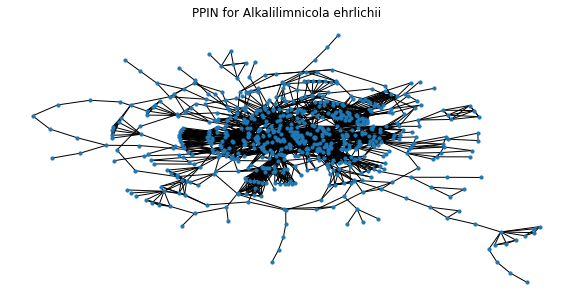
\includegraphics[width=.4\linewidth]{PPIN_fig1}
  \caption{An example PPIN}
  \label{fig:PPIN_fig1}
\end{wrapfigure}

In order to apply common network analysis techniques, we restructured the PPIN data as a series of adjacency matrices. To reduce the computational burden during initial algorithm development, we selected an arbitrary subset of 75 species of Proteobacteria, a major phylum which includes a wide variety of pathogenic genera such as Salmonella. For network statistics that only pertain to connected graphs, we use the largest connected subgraph (or LCSG).

To extract pertinent information about network stability from each network we used the concept of Exponential Random Graph Models. The basic assumption of these models is that the structure in an observed network can be explained by a vector of sufficient statistics which are a function of the observed network. To construct our models, we first need to find the vector of sufficient statistics for each network.

Using functions of NetworkX, a Python library for network analysis, we calculated statistics for each PPIN, including: average degree centrality, number of triangles, modularity, and maximal clique stats for the complete network and for the LCSG. 

\textbf{Average centrality} for a network describes the average number of edges for all nodes. In other words, this statistic describes the average number of connections for all nodes. If a network has a high average degree centrality then we interpret this network as being dense with respect to the number of nodes in the network.

The \textbf{Number of Triangles} statistic counts the number of triangles in the network--we sum up the number of triangles each node is a part of then divide this number by three. A triangle is a set of three nodes where each node has a relationship to the other two--this is sometimes referred to as a 3-clique. Networks that have a large number of triangles tend to be highly interconnected. However, networks that have a low number of triangles turn out to be poorly connected and may suffer from instability.

\textbf{Modularity} is a measure of the structure of networks or graphs which measures the strength of division of a network into modules. Networks with high modularity have dense connections between the nodes within modules but sparse connections between nodes in different modules.

Cliques are fully connected subgraphs, meaning each node in a clique is directly connected to every other node in the clique. Therefore any clique of size $n>1$ necessarily includes ${n \choose n-1}$ sub-cliques. For our network statistics (e.g. \textbf{Clique-Size Mean}) we only measure maximal cliques, i.e. those cliques which are not sub-cliques of a larger clique. Where clique metrics are derived from the LCSG, the metric name is prefixed with ``LCSG''.

\textbf{GiantProportion} is a simple metric that seems to bring unique information into the model. It is the ratio of nodes in the complete graph that are also members of the LCSG, this is \textit{LCSG Node Count} divided by \textit{Total Node Count}.

Additionally, we wrote a function which would find the number of k-stars in each PPIN from one to the maximum size star in the network. For example, a 1-star is the number of nodes in the network, a 2-star is the number of edges, a 3-star is the number of nodes with three edges, and so on. Finally, we combined all of these statistics into a data matrix for our models (see appendix for complete details).

\subsection{Models}
Our research question aims to find network statistics, which measure topological stability of the species’ protein interactome, that are significant predictors of the evolutionary time of a species. That is, we suspect that there is a relationship between some of these network statistics and the response--evolutionary time. The question is, which of the network statistics have the most influence on the response variable? The nature of our data is that there are more variables than data points. Moreover, our network statistics all describe some aspect of topological stability for the network--meaning that they are all highly correlated with each other. For this reason we need models that work well with such data--we need models which perform feature selection, are interpretable, and highly accurate. For this we chose two supervised learning models: LASSO regression and Random Forest regression. 

The LASSO method regularizes model parameters by shrinking the regression coefficients, using the L1 norm, reducing some of them to zero. The feature selection phase occurs after the shrinkage, where every non-zero value is selected to be used in the model. Hence, important network statistics for this model where taken to be those which have non-zero coefficients. While building our initial model we used $\text{alpha} = 0.6$. This is mostly due to convergence issues and will likely change for the final model.

Random forests build a collection of de-correlated decision trees, by randomly choosing only $m$ predictors from the full set of predictors when performing a split, the split is only allowed to use one of those $m$ predictors. Finally, the average of the resulting trees is taken. In random forest regression, features are selected that improve the variance reduction. That is, correlation between trees is reduced without increasing the variance too much. For our initial model we used a max depth of four--a parameter that we plan to tune before choosing a final model.

\section{Preliminary Results}
The network statistics with the most influence on the evolutionary time of each species for the LASSO model were the number of triangles, clique count, LCSG clique count, node count, LCSG node count, LCSG Degree Max, and number of 1-stars (see Figure 2). The sign of coefficients tells you if the network statistic is positively or negatively related to the response, evolutionary time. This project is not focused on finding a linear relationship however we will try to interpret these coefficients.
\begin{wrapfigure}{r}{0.5\textwidth}
  \vspace{-20pt}
  \begin{center}
    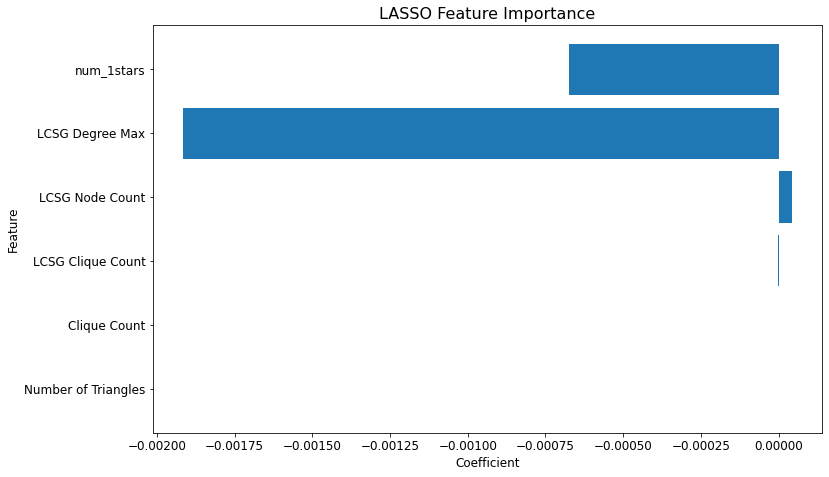
\includegraphics[width=0.48\textwidth]{PPIN_fig3}
  \end{center}
  \vspace{-20pt}
  \caption{LASSO Feature Selection}
  \vspace{-10pt}
\end{wrapfigure}
\indent In Figure 2 we can see that LCSG node count (the number of nodes in the LCSG) and LCSG clique count (the number of maximal cliques in the LCSG) are both positively related to a species' evolutionary time.  Recall that network resilience is the measure of how quickly a network breaks down as edges between nodes are randomly removed and it has been shown that networks with low network resilience also have a low evolutionary time. Hence as the LCSG clique count rises, the LCSG becomes more stable and so we can expect an increase in evolutionary time of the species. On the other hand if the LCSG has a node with a large number of edges (LCSG max degree), those edges only lead to other nodes in the LCSG, meaning that if this number is high then a LCSG in the network has a high density. This may or may not be a good thing for the survival of the species. If this LCSG also had a small amount of nodes then I would assume the evolutionary time would be low but if the number of nodes is high then it may be beneficial. The number of triangles and maximal clique count have been included in the model but the coefficients are close to zero. The mean squared training error for the LASSO model was 0.05. 

The random forest regression model was consistent with the results from above, please see the important variables for this model (See Figure 3). Arguably, the network statistics with the most influence on the evolutionary time of each species for this model were the number of nodes, modularity, clique count, average centrality, LCSG clique-size mean, and a number of other k-stars statistics. 
\begin{wrapfigure}{r}{0.5\textwidth}
  \vspace{-20pt}
  \begin{center}
    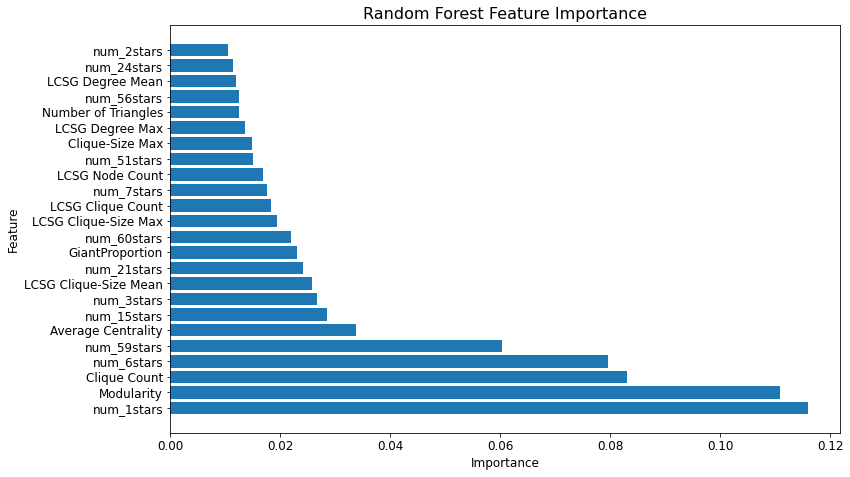
\includegraphics[width=0.48\textwidth]{PPIN_fig2}
  \end{center}
  \vspace{-20pt}
  \caption{Random Forest Feature Selection}
  \vspace{-10pt}
\end{wrapfigure}

We explained before how modularity and average degree centrality influence the topological stability of a network. The LCSG clique-size mean denotes the average size of a maximal clique within the LCSG. If this number is large, then we can expect the stability of this network to be strong and this translates to a higher network resilience. The k-stars statistics are likely to be significant since a network with many high degree nodes would be dense. The mean squared training error for the random forest regression model was 0.009.

\section{Conclusion}
There are many possible confounders which should be considered along with our preliminary results: investigative biases towards modeling common or popular organisms, network size, and genome size. It seems that the network statistics we have found so far and entered into the models do a fair job of describing topological stability. Moreover, many of these statistics do have a significant relationship to evolutionary time of a species. In the next few weeks, we plan to fine-tune the hyperparameters of the models. For example we intend to add cross validation to the LASSO model and use the \textit{RandomizedSearchCV} function to find optimal parameters for the Random Forest model. Additionally, we are implementing a function which will remove a fraction of edges from each network then calculate how many removals it takes for the network to have less than 10 percent of nodes in its largest connected component. 
\section{Appendix}
\subsection{Exhaustive Enumeration of Cliques is Memory-bound}
\begin{wrapfigure}{r}[0pt]{0pt}
\centering
  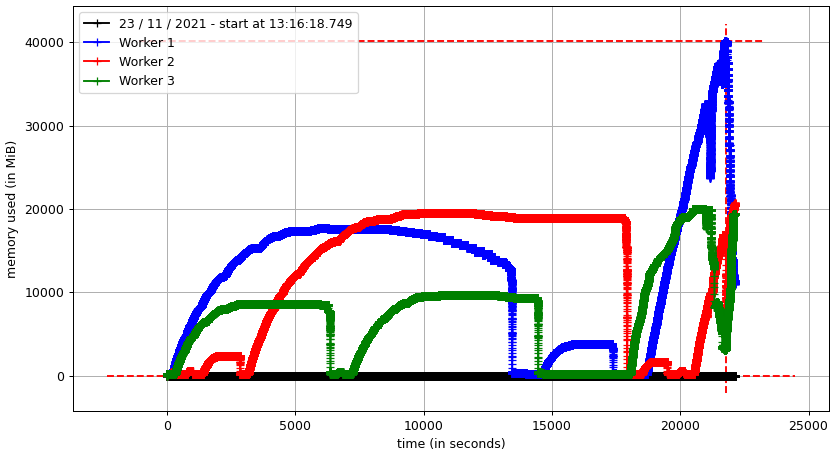
\includegraphics[width=0.4\linewidth]{workers}
  \caption{$Worker$ memory usage}
  \label{fig:workers}
\end{wrapfigure}
We tried implementing exhaustive enumeration of \textit{all} cliques (as opposed to \textit{maximal} cliques) but found this to be impractical, as the supporting NetworkX algorithm (\textit{enumerate\_all\_cliques}) is memory-bound. We tested this limitation via execution with 64GB of RAM and 3 $Worker$ processes; execution failed with a $MemoryError$ after $\sim8$ hours of processing, when one of a workers attempted to allocate additional memory beyond available capacity (see Figure 2).
\subsection{K-Stars Algorithm}
Below is pseudocode for how we constructed the data frame of stars counts for each network.
\begin{algorithm}
\caption{Get Stars Algorithm}\label{alg:cap}
\begin{algorithmic}
\State $\text{LCSG } \gets \text{ giant component for undirected network}$
\State $\text{A } \gets \text{ convert LCSG to adjacency matrix}$
\State $\text{d } \gets \text{ sum row elements of A}$
\State $\text{values, counts } \gets \text{ find unique elements and counts for each}$
\State $\text{stars } \gets \text{ pandas DataFrame of counts with index names being values}$
\end{algorithmic}
\end{algorithm}
\begin{table}[H]
\centering
\caption{Count K-Stars Data Frame}
\begin{tabular}{lrrrrrr}
\toprule
Species\_ID &  882   &  883   &  36870 &  52598 &  56780 & $\cdots$\\
\midrule
num\_1stars &  109.0 &   39.0 &   22.0 &   17.0 &   26.0 & $\cdots$\\
num\_2stars &  105.0 &   57.0 &   54.0 &   30.0 &   70.0 & $\cdots$\\
num\_3stars &   65.0 &   63.0 &   31.0 &   20.0 &   53.0 & $\cdots$\\
$\vdots$ &   $\vdots$ &   $\vdots$ &   $\vdots$ &    $\vdots$ &   $\vdots$ & $\ddots$\\
\bottomrule
\end{tabular}
\end{table}
It is important to note that the maximum star count is unique to each network so when we concatenate these smaller data frames together to form the data frame which holds all network statistics it must be dynamic. Additionally, this means that once we train the model--if we choose to include all star variables--then we cannot test the model on a new set of networks. A quick fix for this may be to only include the first ten rows of this data frame.
\subsection{Predictors Using NetworkX}
\begin{table}[H]
\centering
\caption{Predictors Using NetworkX Data Frame}
\begin{tabular}{lrrrrrr}
\toprule
Species\_ID &      882   &     883   &    36870 &    52598 &      56780 & $\cdots$ \\
\midrule
Average Centrality    &      0.013 &     0.019 &    0.023 &    0.030 &      0.020 & $\cdots$ \\
Number of Triangles   &  12742.000 &  8017.000 &  689.000 &   49.000 &  11135.000 & $\cdots$\\
Modularity            &      0.679 &     0.559 &    0.674 &    0.741 &      0.556 & $\cdots$\\
Clique Count          &   1060.000 &  3580.000 &  209.000 &  823.000 &    547.000 & $\cdots$\\
Clique-Size Max       &     26.000 &    19.000 &   10.000 &    6.000 &     27.000 & $\cdots$\\
Clique-Size Mode      &      2.000 &     5.000 &    2.000 &    2.000 &      2.000 & $\cdots$\\
Clique-Size Mean      &      4.726 &     5.004 &    2.923 &    2.335 &      4.075 & $\cdots$\\
LCSG Clique Count     &    916.000 &   371.000 &  180.000 &  249.000 &    451.000 & $\cdots$\\
LCSG Clique-Size Max  &     26.000 &    19.000 &   10.000 &    5.000 &     27.000 & $\cdots$\\
LCSG Clique-Size Mode &      2.000 &     2.000 &    2.000 &    2.000 &      2.000 & $\cdots$\\
LCSG Clique-Size Mean &      5.102 &     4.647 &    3.039 &    2.116 &      4.237 & $\cdots$\\
LCSG Node Count       &    736.000 &   502.000 &  217.000 &  139.000 &    536.000 & $\cdots$\\
LCSG Degree Max       &     60.000 &    58.000 &   27.000 &   11.000 &     66.000 & $\cdots$\\
LCSG Degree Mode      &      1.000 &     3.000 &    2.000 &    2.000 &      2.000 & $\cdots$\\
LCSG Degree Mean      &      9.465 &     9.661 &    5.060 &    4.144 &     10.590 & $\cdots$\\
\bottomrule
\end{tabular}
\end{table} \newpage
\begin{thebibliography}{1}
 \bibitem{1} Zitnik, M., Sosič, R., Feldman, M. W., Leskovec, J. (2019). Evolution of resilience in protein interactomes across the tree of life. Proceedings of the National Academy of Sciences, 116(10), 4426-4433. \url{https://doi.org/10.1101/454033}
\bibitem{2} Maddamsetti, R. (2021). Selection maintains protein interactome resilience in the long-term evolution experiment with Escherichia coli. \url{https://doi.org/10.1093/gbe/evab074}
\bibitem{3} Evolution of protein interactomes across the tree of life. (n.d.). Retrieved from \url{http://snap.stanford.edu/tree-of-life/}
\bibitem{4} Sumit Mukherjee. (2011). Exponential Random graph models. Retrieved from \url{https://artowen.su.domains/courses/319/smukherjee.pdf}
  \end{thebibliography}

%%%%%%%%%%%%%%%%%%%%%%%%%%%%%%%%%%%%%%%%%%%%%%%%%%%%%%%%%%%%%%%%%%%%%%%%%%%%%
\end{document}
